\section{Model}
This section introduces the architecture details of our network. Section~\ref{sec:model:transducer} discusses the high-level design of the network. Then Section~\ref{sec:model:encoder} introduces our convolutional encoder, the most important contribution of this paper. Later Section~\ref{sec:model:encoder_efficiency} discusses how we progressively reduce the temporal length of the input utterance in the network to reduce the computation while maintaining the accuracy. This section concludes with the discussion on model scaling. 

\subsection{End-to-end network: CNN-RNN-Transducer}
\label{sec:model:transducer}
Our network design is based on the RNN-Transducer framework \cite{graves2012sequence, rao2017exploring, he2017streaming}. The network contains three components: audio encoder on the input utterance, label encoder on the input label and a joint network to combine the two and decode. 

We directly use the label encoder and the joint network from \cite{zhang2020transformer}, but propose a new CNN based audio encoder. 

\subsection{Encoder design}
\label{sec:model:encoder}
Let the input sequence be $x^0=(x_1, \ldots, x_T)$ where $T$ is the temporal length of the sequence and $x_i \in\mathbb{R}^N$ is the $N$ dimensional features of each audio frame. The audio encoder operates on $x^0$ and outputs a sequence of encoded features $y=(y_1, \ldots, y_{T'})$ where $y_j\in\mathbb{R}^{N'}$ and $T'$ is the encoded length. Note that here $T'\ne T$ because the audio encoder reduces the length of sequence. To make it formal, let $\mathrm{AudioEncode}(\cdot)$ be the encoding function, we have
\begin{equation}
    (y_1, \ldots, y_{T'}) = \mathrm{AudioEncode}(x_1, \ldots, x_T).
\end{equation}

$y=(y_1, \ldots, y_{T'})$ will be the input to the RNN-T decoder.

We design the $\mathrm{AudioEncode}(\cdot)$ function via stacking multiple blocks of convolutions. Let $\mathrm{C}_k$ represent the $k$-th block of convolution, and let $x^k = \mathrm{C}_{k}(x^{k-1})$. We have
\begin{equation}
\begin{split}
    y = \mathrm{AudioEncode}(x) = \mathrm{C}_K\left(\mathrm{C}_{K-1}\left(\ldots \mathrm{C}_{1}(x)\right)\right)
\end{split}
\end{equation}

Each $\mathrm{C}(\cdot)$ includes five layers of convolution operations, each followed by batch normalization~\cite{goodfellow2016deep} and an activation function. It also contains the skip connection~\cite{he2016deep} as well as the squeeze-and-excitation component~\cite{hu2018squeeze}. Let $m$ represents the number of convolution layers of a block. Let $\mathrm{Conv}$ represent the 1D convolution. Let $\mathrm{SE}$ represent the squeeze-and-excitation module. Under this notation, we have

\begin{equation}
\begin{split}
&\mathrm{C}(x) = \mathrm{SE}\left(f^{m-1}\left(f'(x)\right)\right) + x,\\
&f(x)=\mathrm{Act}(\mathrm{BN}(\mathrm{Conv}(x)))
\end{split}
\end{equation} where $f^m$ means stacking $m$ layers of the function $f(\cdot)$ on the input. Inside each block, the first layer $f'$ can be different from the rest $m-1$ layers $f$ in the number of input and output convolution channels as well as the convolution stride. In addition, $\mathrm{Act}$ represents the activation function, and we've tried both ReLU and swish function~\cite{ramachandran2017searching}. For reader's convenience, we repeat the definition of the swish function here:
\begin{equation}
f(x)=x\cdot \sigma(\beta x)=\frac{x}{1+\exp{\left(-\beta x\right)}},
\end{equation}
where $\beta$ is a trainable parameter. We've observed that the swish function works slightly better than ReLU. Figure~\ref{fig:conv_block} illustrates the block.

\begin{figure}
    \centering
    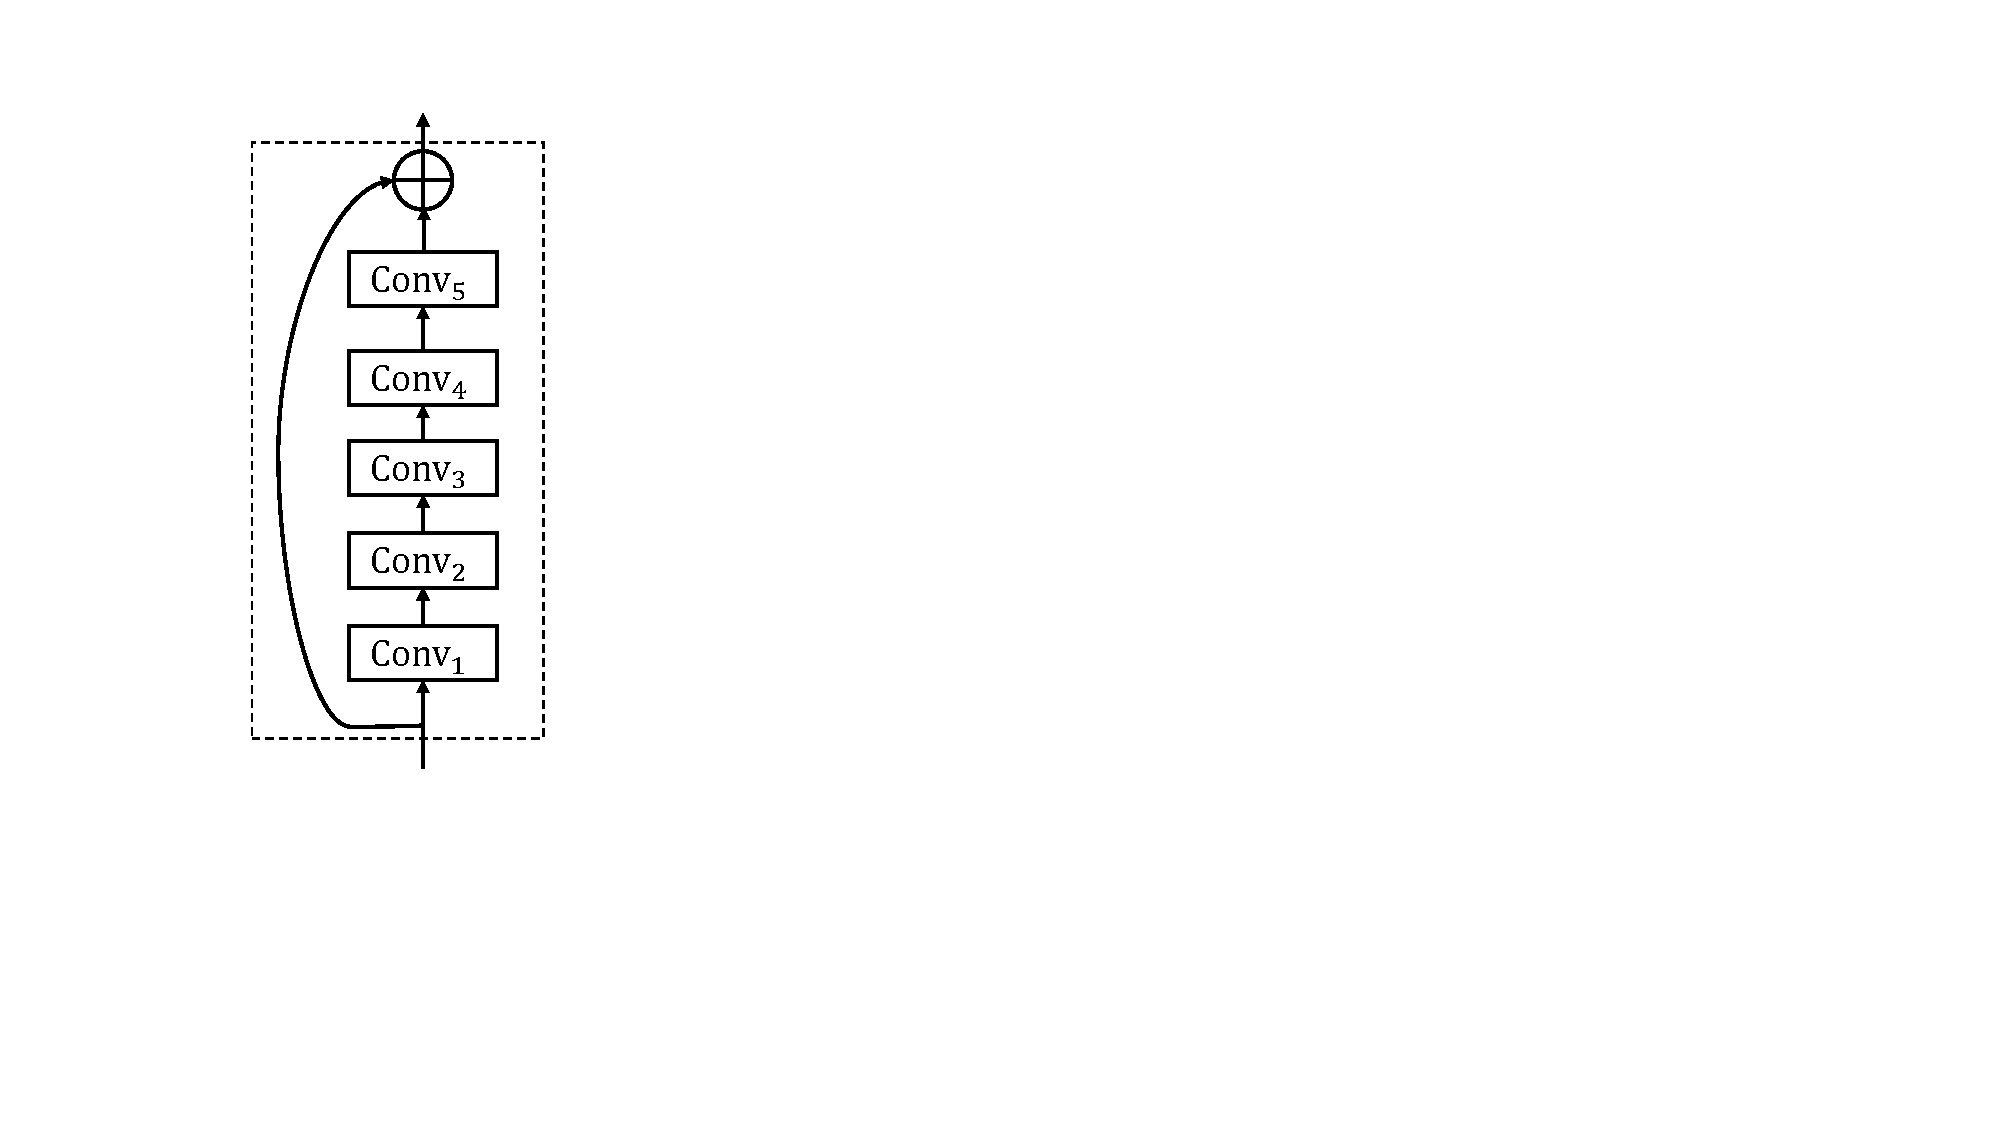
\includegraphics[width=0.3\columnwidth]{LaTeX/figure/skip.pdf}
    \caption{A convolution block $C_i$ contains a number of convolutions, each followed by squeeze-and-excitation, batch normalization and activation. Skip connection is applied on the output of the final convolution layer.}
    \label{fig:conv_block}
\end{figure}

The Squeeze-and-excitation~\cite{hu2018squeeze} function $\mathrm{SE}(\cdot)$ performs global average pooling on the input $x$ and transforms it into a global channelwise weight $\theta(x)$ and element wise multiply each frame by this weight. We adopt the idea to the 1D case, to be precise,
\begin{equation}
\begin{split}
    \bar{x}&=\frac{1}{T} \sum_{t} x_t\\
    \theta(x)&=\mathrm{Sigmoid}(W_2(\mathrm{Act}(W_1\bar{x} + b_1)) + b_2) \\
    \mathrm{SE}(x)&=\theta(x)\circ x \\
\end{split}
\end{equation}
where $\circ$ means element-wise multiplication. If $x\in\mathbb{R}^d$, we have $W_1\in\mathbb{R}^{d\times d/8}$, and $W_2\in\mathbb{R}^{d/8 \times d}$. Note that $\mathrm{Sigmoid}(\cdot)$ maps its input to $(0, 1)$.

Figure~\ref{fig:squeeze_and_excitation} illustrates the squeeze-and-excitation function.
\begin{figure*}
    \centering
    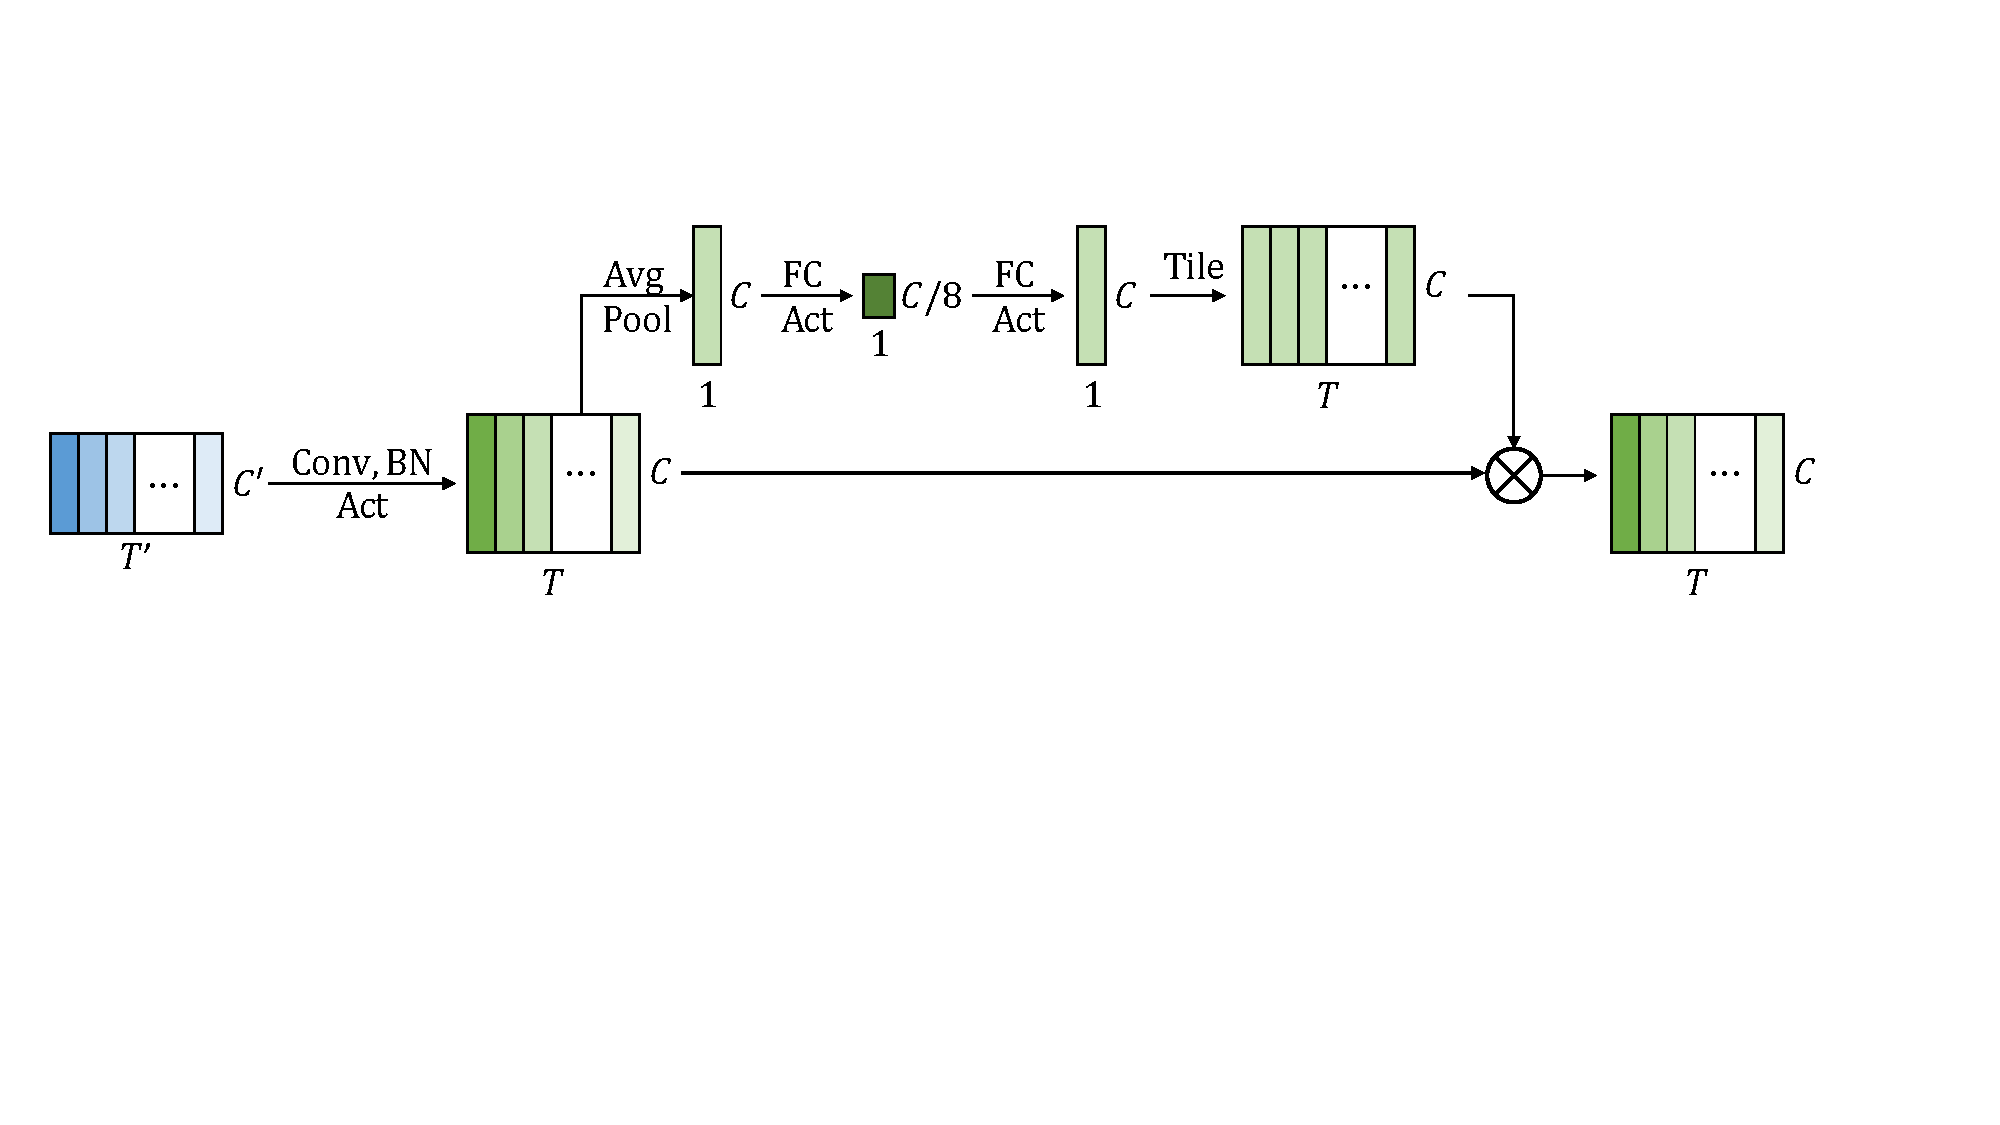
\includegraphics[width=0.8\textwidth]{LaTeX/figure/SqueezeAndExcitation.pdf}
    \caption{1D Squeeze-and-excitation module. The input first goes through a convolution layer followed by batch normalization and activation. Then average pooling is applied to condense the conv result into a 1D vector, which is then processed by a bottleneck structure formed by two fully connected (FC) layers with activation functions. The output goes through a Sigmoid function to be mapped to $(0, 1)$, and then tiled and applied on the conv output using pointwise multiplications.}
    \label{fig:squeeze_and_excitation}
\end{figure*}

In our final design, the network has $17$ convolution blocks $C_0, \ldots, C_{16}$. Except $C_0$ and $C_{16}$ which only have one layer of convolution each, all the other convolution blocks have $5$ layers of convolution.

\subsection{Encoder efficiency}
\label{sec:model:encoder_efficiency}
\subsubsection{Progressive downsampling} We use a convolution layer of stride two to reduce the temporal length of the signal by half. In contrast to the previous CNN models that only downsample the input signal at the first layer only, we progressively apply downsampling at three different convolution blocks layers of the network, leading to in a total reduction factor of eight on the input signal. See Figure~\ref{fig:downsampling} for an illustration. This enables significant computation reduction since the computation cost of 1D convolution scales linearly with respect to the temporal length of the input signal. This avoids loss of information at an early stage. In addition, we include a few blocks of convolutions between two consecutive downsampling layers, allocating enough network capacity to extract rich information at a scale. As a result of this careful design, we observe no loss of accuracy when we put the encoder to the RNN-T framework. Section~\ref{sec:experiments} will validate this in experiments.

\begin{figure}
    \centering
    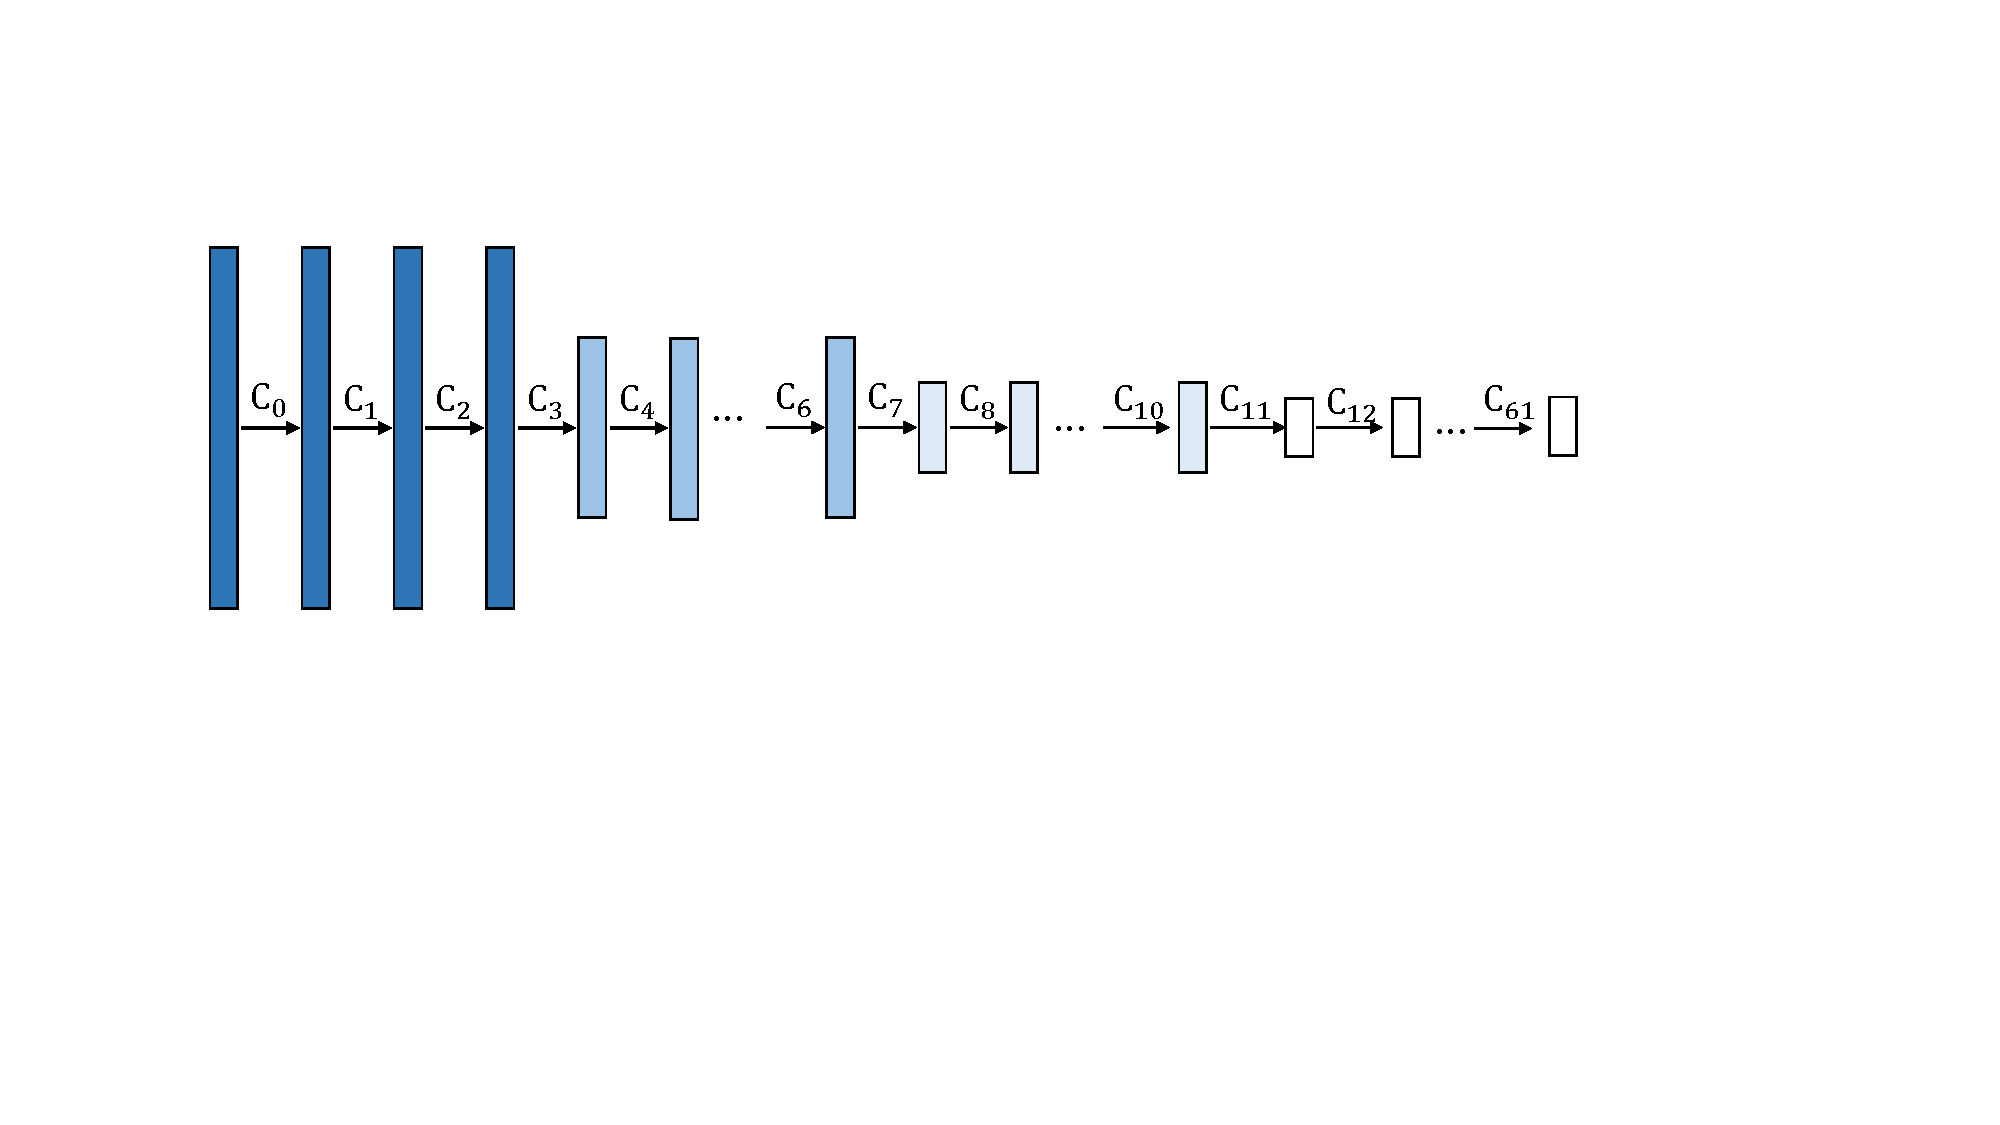
\includegraphics[width=0.9\columnwidth]{LaTeX/figure/Downsample.pdf}
    \caption{The encoder progressive downsamples the input utterance.}
    \label{fig:downsampling}
\end{figure}

\subsubsection{Small filter size} One of the claim from previous CNN works \cite{li2019jasper,kriman2019quartznet} is that larger filter size of the convolution layers benefit the encoder. In contrary, we set the filter size of every single convolution layer in our net to as small as five, and we observe significant improvement on the WER on LibriSpeech test clean. We suspect that the cause of this conter intuitive phenomenon is the effecitve receptive field of an encoder output node; when an output node covers too long segment of the input audio, the model overfits.

To analyze this more, we follow a previous work~\cite{luo2016understanding} and plot the normalized effective receptive field of our model compared against Jasper and QuartzNet in Figure~\ref{fig:yy} before training. We choose $4\sigma$ as the effective receptive field, and observe that the effective receptive field of our model is the smallest among all. Nevertheless, each encoder output covers $2-3$ seconds of audio, which is long enough to contain the pronunciation of a few words. This empirically demonstrates that our choice of small filter size reduces the risk of overfiting; nevertheless the receptive field is big enough to extract rich information from a long enough sequence of local neighboring audio.

\subsection{Model scaling}
Except for the final convolution layer, we allow the number of input channels and the number of output channels of our model to scale linearly with respect to a hyper parameter $\alpha$. Tuning $\alpha$ linearly affects the number of parameters as well as the flops. Due to the finding about the filter size in the previous section, we do not scale the filter size. This is different from EfficientNet which scales more than one design factors together.

Table \ref{tab:xx} summarizes the architecture details of our network. 

\begin{table}[!tb]
    \centering
    \begin{tabular}{ccccc}
        \hline
         Block ID & \makecell{\# Conv \\ Layers} & \makecell{\#Output \\channels} & \makecell{Filter \\ size} & other \\ \hline\hline
         $C_0$ & 1 & 256 & 5 & No residual \\ \hline
         $C_1$-$C_{10}$ & 5 & 256 & 5 & stride of $C_4, C_7$ is $2$\\ \hline
         $C_{11}$-$C_{29}$ & 5 & 512 & 5 & stride of $C_{11}$ is $2$ \\ \hline
         $C_{30}$ & 1 & 640 & 5 & dilation is $2$\\ \hline
    \end{tabular}
    \caption{Configuration of the network}
    \label{tab:table}
\end{table}


% \section{Relationship with the previous works}

% CNN models in speech
% Our work is inspired many previous work on using the CNN 

% ASR models

% CNN models in vision(weihan)

% \paragraph{CNN models in speech}

% Group 2: 
